\part[Projektdokumentation]{Projektdokumentation
                  \begin{center}
                     \begin{minipage}[c]{10.7cm}
                      \small Hitobito: Neue Generation von Personen-Filtern \\
                      Autor: Marc Egli
                     \end{minipage}
                  \end{center}
                 }
\chapter{Einführung}
Puzzle ITC ist ein schweizer Anbieter für Softwarelösungen. Die Firma hat ihren Hauptsitz in Bern,
besitzt aber weitere Standorte in Zürich, Luzern und Deutschland (Thüringen). Puzzle bietet als Unternehmen
die ganze Palette an IT-Services an, von Digital Transformation bis hin zu Data Analytics. Nebst den vielen Angeboten
tritt Puzzle dabei immer seine Grundwerte nach aussen, welche im Puzzlehouse abgebildet werden.

\begin{figure}[h]
   \centering
   
\includegraphics[width=1\textwidth,]{puzzle-house.png}
   \caption{Rollen in Scrum}
\end{figure}

Hitobito ist eines der Angebote von Puzzle. Es ist ein Community-Management Tool und
als Open-Source Projekt auf Github zu finden. Das Tool wird von zahlreichen Verbänden, Parteien
und Organisationen verwendet und befindet sich darum in einer kontinuerilichen Weiterentwicklung. Mit dem Wagons-Gem
ermöglicht es Hitobito zudem spezielle Kundenanpassungen in einem eigenen "Wagon" zu vollziehen, ohne die Software anderer
Kunden mit-anzupassen.

Ich selbst arbeite jetzt seit einem halben Jahr im Hitobito und nahm darin vor allem Upgrades und Migrationen vor. So durfte ich
bspw. das Upgrade von RoR (Ruby on Rails) von 6.1 auf 7.1 vornehmen oder die Migration von MySQL auf Postgres vollziehen.

Da Hitobito von zahlreichen Kunden verwendet wird, ist die Applikation über die Jahre gewachsen. Viele Features wurden implementiert,
um sie schnell dem Kunden zur Verfügung zu stellen. Mit einem immer wachsenden Anforderungskatalog ergaben sich dadurch komplexe Arbeitsabläufe
welche im Tool etabliert wurden. Einer dieser komplexen Abläufe ist die Filterung nach Personen oder Abonnemente.

Mit dieser IPA soll die Filterung zwischen diesen zwei Entitäten homogenisiert werden. Um dies zu tun,
sollen zuerst zwei bis drei Konzepte ausgearbeitet und anschliessend in einem Variantenentscheid evaluiert werden. Für die Lösungsvariante wird in einem weiteren Schritt ein PoC (Proove of Concept) implementiert. 

Nach der IPA soll basierend auf der neuen Filterlogik ein neues UI entworfen werden, um nebst der Ordnung im Backend
eine besser User Experience für den Benutzer zu schaffen.

In einer Zeit in welcher Unternehmen mehr den je Wert auf ein sauberes Design und der User Experience von Webseiten und Applikationen geben, das auch
in einer älteren Applikation zu etablieren. Gerade bei einem Community-Management Tool wie Hitobito, welches tagtäglich von 
Personen bedient werden, welche nicht das technische Know-How dahinter besitzen, ist es wichtig Arbeitsabläufe so einfach wie möglich zu entwerfen, um 
maximale Effizienz für diese Personen zu garantieren. Durch eine Vereinfachung der Hitobito-Fitler machen wir damit einen ersten Schritt in die richtige
Richtung.

\chapter{Analyse}
In der Analyse der IPA wird der Rahmen geschaffen in welchem man später während des Implementierens arbeitet. 
Sie befasst sich mit der Aufnahme von Ist- und Zielzustand und definierte Funktionale sowie nicht funktionale Anforderungen.
Es wird definiert wo sich die IPA abgrenzt. 

\section{Ist-Zustand}

\subsection{Personenlisten}
Aktuell kann ein Nutzer über den Button Neuer-Filter auf die Filter Seite navigieren. 
\begin{figure}[h]
   \centering
   \fbox{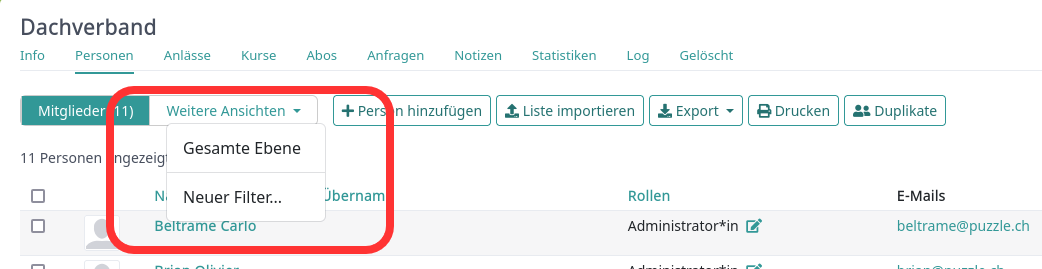
\includegraphics[width=1\textwidth,]{hitobito_header.drawio.png}}
   \caption{Hitobito Personenlisten Filtererstellung}
\end{figure}

\newpage 

Auf dieser definiert er die Filterungskriterien für die Attribute Rollen, Qualifikationen,
Felder, Sprache und Tags. 
\begin{figure}[h]
   \centering
   \fbox{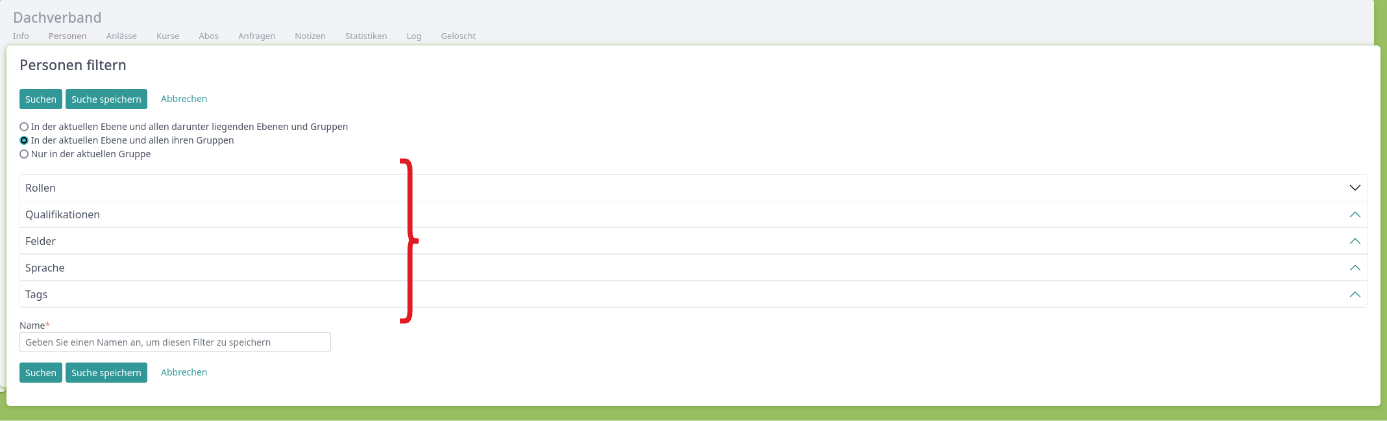
\includegraphics[width=1\textwidth,]{hitobito_person_list_filter.drawio.png}}
   \caption{Hitobito Personenlisten Filterkriterien}
\end{figure}

Anschliessend ist es dem Nutzer möglich seinen Filter über einen Button für die Wiederverwendung
zu speichern.
\begin{figure}[h]
   \centering
   \fbox{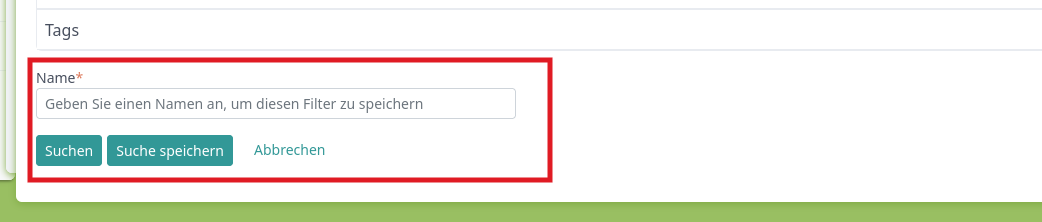
\includegraphics[width=1\textwidth,]{save_filter.drawio.png}}
   \caption{Hitobito Personenlistenfilter Speicherung}
\end{figure}

\newpage

Technisch sind die Personenlisten-Filter nach folgendem Sequenzdiagramm aufgebaut:
\begin{figure}[h]
   \centering
   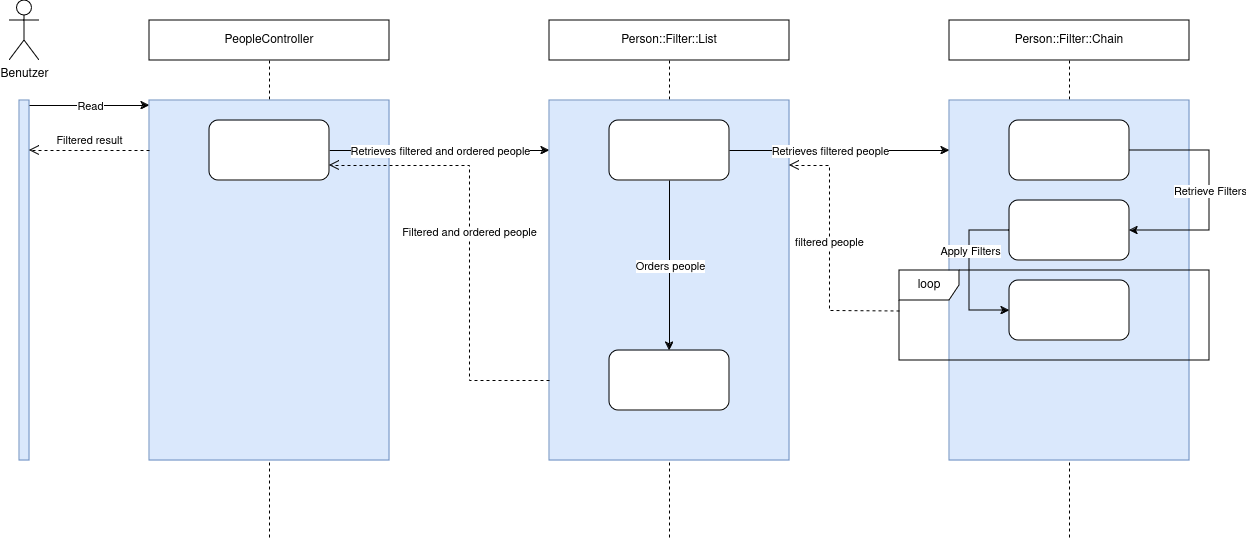
\includegraphics[width=1\textwidth,]{person_filter.png}
   \caption{Sequenzdiagramm Personenlisten Filter}
\end{figure}

\begin{table}[h!]
   \begin{tabular}{|L{0.4\textwidth}|L{0.5\textwidth}|}
       \hline
       \rowcolor{puzzleblue} \multicolumn{2}{|l|}{\color{white}\textbf{Beschreibung Sequenzdiagramm}} \\[12pt]
       \hline
       PeopleController & Der PeopleController nimmt den Request des Benutzers entgegen und erwidert die gefilterten und sortierten Personen auf welche der Benutzer zugreifen darf. \\
       \hline
       Person::Filter::List & Personen auf welche der Benutzer keinen Zugriff hat werden rausgefiltert und anschliessend sortiert. \\
       \hline
       Person::Filter::Chain & Definiert anhand der Request Parameter vom Controller die Filter und wendet diese in einem Loop via chain-pattern an. \\
       \hline
     \end{tabular}
     \caption{Beschreibung Sequenzdiagramm}
\end{table}

\newpage

\subsection{Abonnemente}
Auf den Abonnementen kann der Nutzer Filterkriterien in den globalen Bedingungen definieren.

\begin{figure}[h]
   \centering
   \fbox{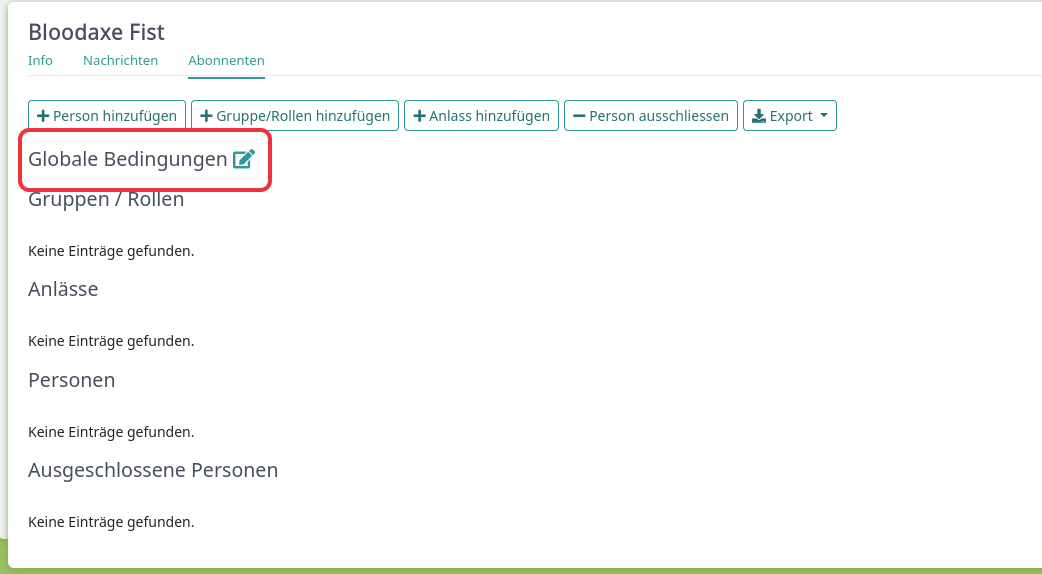
\includegraphics[width=1\textwidth,]{hitobito_global_conditions.drawio.png}}
   \caption{Hitobito Globale Bedingungen}
\end{figure}

Unter diesen kann der Nutzer per Dropdown entscheiden für welche Attribute er die Filterkriterien definieren möchte.
Er kann auch bereits gesetzte Kriterien entfernen. Pro Filterkriterium entscheidet er im weiteren, mit welcher Genauigkeit
nach diesem Filterkriterium gesucht wird. Bei Zahlen ist es möglich die Genauigkeiten ist genau, ist höher als und ist kleiner als 
einzustellen. Bei Textvergleichen sind es ist genau, enthält, enthält nicht.
\begin{figure}[h]
   \centering
   \fbox{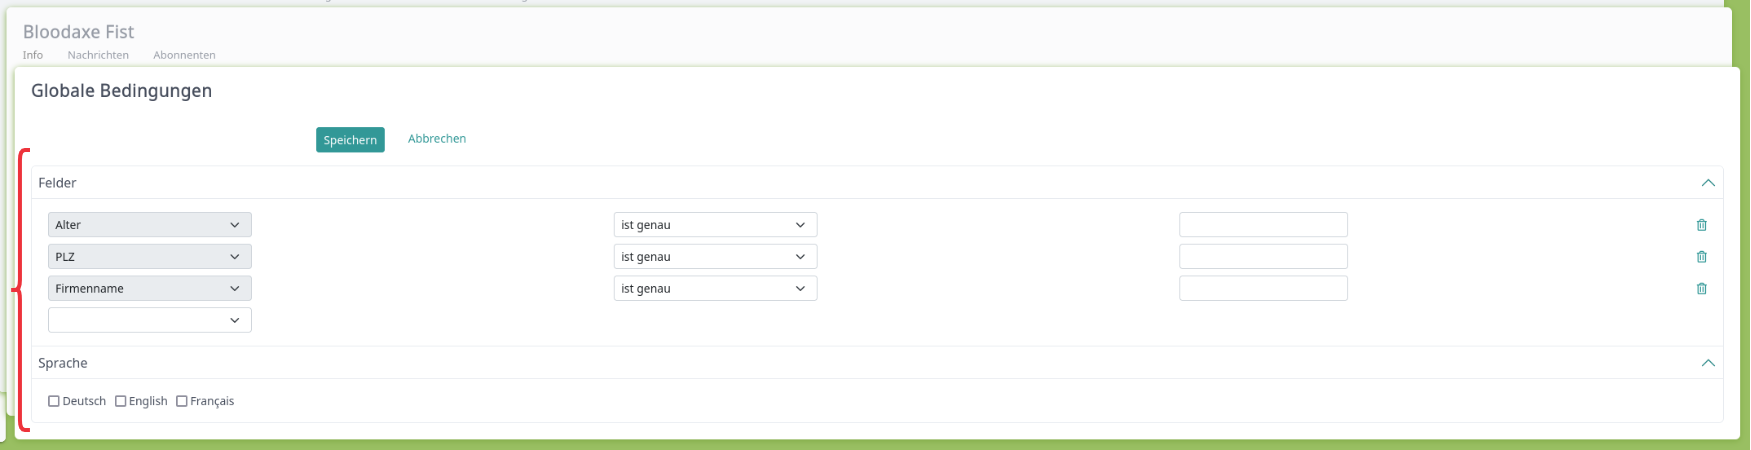
\includegraphics[width=1\textwidth,]{hitobito_filter_conditions.drawio.png}}
   \caption{Hitobito Filterkriterien}
\end{figure}

\newpage

Hat der Nutzer seine Filterkriterien und die dazugehörigen Genauigkeiten definiert, kann er sie über den
Speicher-Button persistieren. Im Anschluss werden die ausgewählten Filterkriterien in den Globalen Bedingungen angezeigt
und ein Success-Alert ausgelöst der die Aktualisierung bestätigt.
\begin{figure}[h]
   \centering
   \fbox{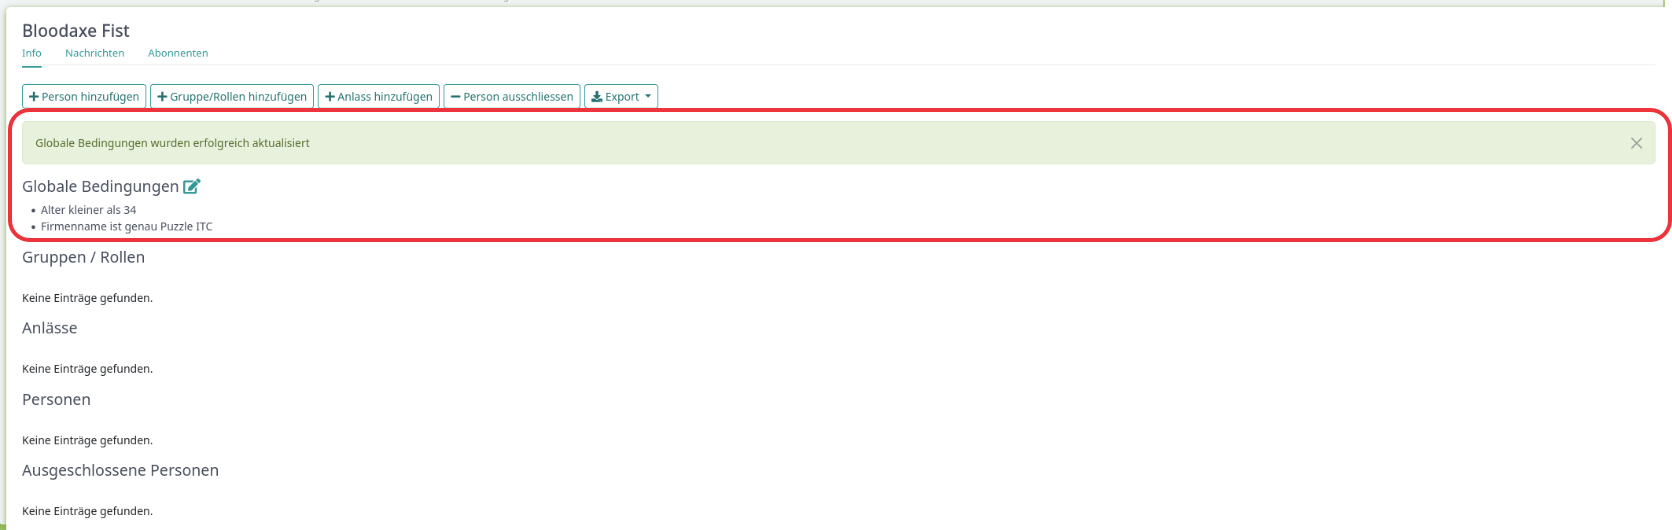
\includegraphics[width=1\textwidth,]{hitobito_filter_created.drawio.png}}
   \caption{Hitobito Filterkriterien}
\end{figure}

Technisch haben sind die Abonnemente nach folgendem ERD aufgebaut.
\begin{figure}[h]
   \centering
   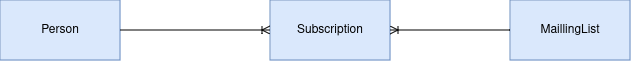
\includegraphics[width=1\textwidth,]{subscriptions_erd.drawio.png}
   \caption{Hitobito Subscription ERD}
\end{figure}

Es ist zu beachten: Eine Person kann mehrere Subscriptions besitzen und jede Subscriptions ist einer
Mailling list zugerodnet. Somit muss bei der Filterung nach Subscriptions zuerst die MaillingList included
werden, damit man auf dieser danach die Filterung ausführen kann.

\newpage

Die Globalen Filterungskriterien für die Abonnemente werden in dem Modell der MaillingList
abgespeichert. Dadurch ergibt sich folgendes Sequenzdiagramm.
\begin{figure}[h]
   \centering
   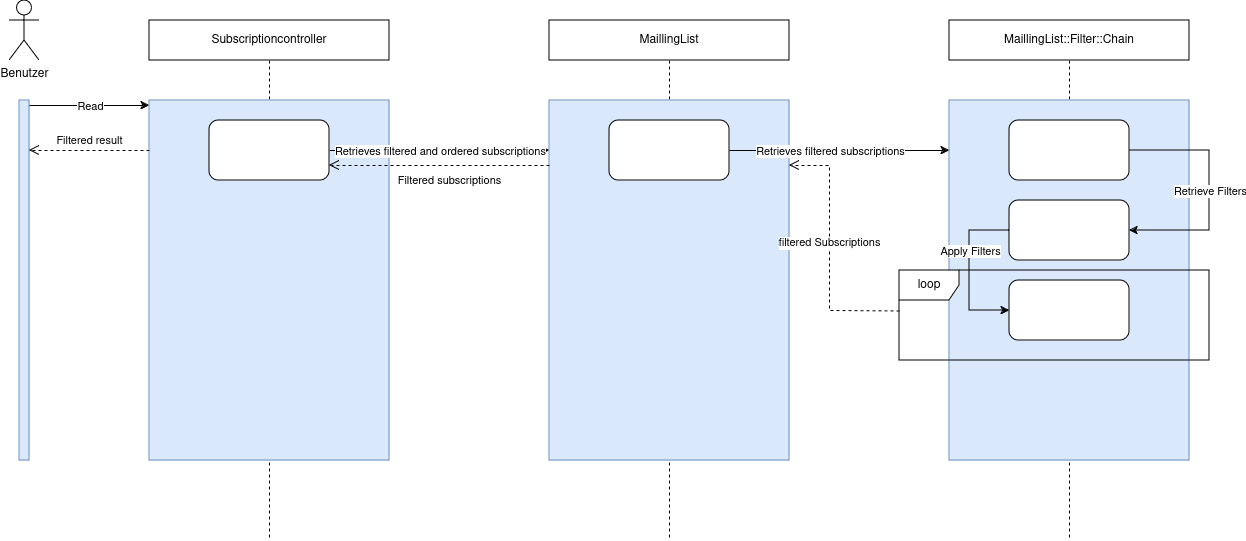
\includegraphics[width=1\textwidth,]{subscriptions_filter.drawio.png}
   \caption{Hitobito Abonnementen Sequenzdiagramm}
\end{figure}

\begin{table}[h!]
   \begin{tabular}{|L{0.4\textwidth}|L{0.5\textwidth}|}
       \hline
       \rowcolor{puzzleblue} \multicolumn{2}{|l|}{\color{white}\textbf{Beschreibung Sequenzdiagramm}} \\[12pt]
       \hline
       SubscriptionController & Der SubscriptionController nimmt den Request des Benutzers entgegen und erwidert die gefilterten und sortierten Personen auf welche der Benutzer zugreifen darf. \\
       \hline
       MaillingList & Fetcht Subscriptions aus der Datenbank und macht Aufruf zum MaillingList::Filter::Chain \\
       \hline
       MaillingList::Filter::Chain & Holt die Filterkriterien aus der Datenbank und filtered die Subscriptions danach aus. \\
       \hline
     \end{tabular}
     \caption{Beschreibung Sequenzdiagramm}
\end{table}

\section{Soll-Zustand}
Das neue Konzept für die Abonnementen- und Personenlistenfilterung soll durch den gleichen Prozess laufen. 
Die beiden Filterungsprozesse sollen dabei zu einem homogenisiert werden und trotzdem die gleichen Funktionalitäten bieten.
Bestehende Datenmodelle sollen ebenfalls fusioniert werden.

\section{Persönliche Vorgehensziele}
\begin{table}[h!]
   \begin{tabular}{|L{0.4\textwidth}|L{0.5\textwidth}|}
       \hline
       \rowcolor{puzzleblue} \multicolumn{2}{|l|}{\color{white}\textbf{Zeitrahmen}} \\[12pt]
       \hline
        Beschreibung & Der erstellte Zeitplan, Meilensteine und Sprints werden erfolgreich eingehalten. \\
       \hline
       Messbarkeit & Die IPA wird komplett und in der definierten Frist abgeben. \\
       \hline
     \end{tabular}
     \caption{Zeitrahmen}
\end{table}

\begin{table}[h!]
   \begin{tabular}{|L{0.4\textwidth}|L{0.5\textwidth}|}
       \hline
       \rowcolor{puzzleblue} \multicolumn{2}{|l|}{\color{white}\textbf{Filterprozesse}} \\[12pt]
       \hline
       Beschreibung & Die Verständnis der Hitobito Filterlogik wird vertieft. \\
       \hline
       Messbarkeit & Zukünftig dient Kandidate als Anlaufstelle für Fragen zur Filterung und
       kann dieses Wissen in anderen Aufträgen anwenden. \\
       \hline
     \end{tabular}
     \caption{Filterprozesse}
\end{table}

\begin{table}[h!]
   \begin{tabular}{|L{0.4\textwidth}|L{0.5\textwidth}|}
       \hline
       \rowcolor{puzzleblue} \multicolumn{2}{|l|}{\color{white}\textbf{Ruby on Rails}} \\[12pt]
       \hline
       Beschreibung & Das Wissen rund um das Ruby on Rails Framework und Aufbau von Domain und Modellklassen 
       wird vertieft. \\
       \hline
       Messbarkeit & Erlangtes Wissen kann in zukünftiger Entwicklung an Features eingesetzt werden. \\
       \hline
     \end{tabular}
     \caption{Ruby on Rails}
\end{table}

\begin{table}[h!]
   \begin{tabular}{|L{0.4\textwidth}|L{0.5\textwidth}|}
       \hline
       \rowcolor{puzzleblue} \multicolumn{2}{|l|}{\color{white}\textbf{Konzeption}} \\[12pt]
       \hline
       Beschreibung & Der Kandidat ist in der Lage Features oder Umstrukturierungen an einer Applikation
       selbständig zu konzipieren. \\
       \hline
       Messbarkeit & Konzept für neues Filterverhalten wurde sauber aufgestell und Entscheidung dafür begründet.  \\
       \hline
     \end{tabular}
     \caption{Konzeption}
\end{table}

\section{Anforderungen}
\subsection{Nicht funktionale Anforderungen}

\begin{table}[h!]
   \begin{tabular}{|L{0.3\textwidth}|L{0.6\textwidth}|}
       \hline
       \rowcolor{puzzleblue} \multicolumn{2}{|l|}{\color{white}\textbf{Erweiterbarkeit, NfA. 1}} \\[4pt]
       \hline
       Beschreibung & Bei der Implementation der neuen Filterlogik wird beachtet, dass zukünftig weitere
       Filterkriterien oder Genauigkeiten vom Kunden gewünscht werden können. \\
       \hline
       Messbarkeit & Die Implementation wurde nachhaltig umgesetzt und bietet Möglichkeiten zur Erweiterung.  \\
       \hline
     \end{tabular}
     \caption{Erweiterbarkeit}
\end{table}

\begin{table}[h!]
   \begin{tabular}{|L{0.3\textwidth}|L{0.6\textwidth}|}
       \hline
       \rowcolor{puzzleblue} \multicolumn{2}{|l|}{\color{white}\textbf{Performance, NfA. 2}} \\[4pt]
       \hline
       Beschreibung & Die Implementation des neuen Filterungskonzeptes soll die gleiche
       Leistungsfähigkeit wie die jetztige Implementation vorweisen. \\
       \hline
       Messbarkeit & Ladezeit der Personenlisten und Abonnemente bleibt gleich.  \\
       \hline
     \end{tabular}
     \caption{Performance}
\end{table}

\begin{table}[h!]
   \begin{tabular}{|L{0.3\textwidth}|L{0.6\textwidth}|}
       \hline
       \rowcolor{puzzleblue} \multicolumn{2}{|l|}{\color{white}\textbf{Security, NfA. 3}} \\[4pt]
       \hline
       Beschreibung & Filterungen sollen auf dem Datensatz gemacht werden, welche durch das can-can-can
       Gem verfiziert hat. \\
       \hline
       Messbarkeit & Nutzer können keine Daten einsehen, auf welche sie keine Berechtigungen haben.  \\
       \hline
     \end{tabular}
     \caption{Security}
\end{table}

\begin{table}[h!]
   \begin{tabular}{|L{0.3\textwidth}|L{0.6\textwidth}|}
       \hline
       \rowcolor{puzzleblue} \multicolumn{2}{|l|}{\color{white}\textbf{DRY, NfA. 4}} \\[4pt]
       \hline
       Beschreibung & Der Code wurde nach dem DRY (Don't Repeat Yourself) Prinzip implementiert. \\
       \hline
       Messbarkeit & Es finden sich keine doppelten Klasse oder unnötige Wrapper.  \\
       \hline
     \end{tabular}
     \caption{DRY}
\end{table}

\newpage

\begin{table}[h!]
   \begin{tabular}{|L{0.3\textwidth}|L{0.6\textwidth}|}
       \hline
       \rowcolor{puzzleblue} \multicolumn{2}{|l|}{\color{white}\textbf{Dokumentation, NfA. 5}} \\[4pt]
       \hline
       Beschreibung & Code wurde dokumentiert. \\
       \hline
       Messbarkeit & Codingfiles sind mit verständlichen Kommentaren versehen.  \\
       \hline
     \end{tabular}
     \caption{Dokumentation}
\end{table}
 
\subsection{Funktionale Anforderungen}
\begin{table}[h!]
   \begin{tabular}{|L{0.3\textwidth}|L{0.6\textwidth}|}
       \hline
       \rowcolor{puzzleblue} \multicolumn{2}{|l|}{\color{white}\textbf{Konzept, fA. 1}} \\[4pt]
       \hline
       Beschreibung & Das erstellte Konzept führt beide Filterprozesse zusammen. \\
       \hline
       Messbarkeit & Es gibt im Hitobito ein homogenisierter Fitlerprozess der für weiter Filterungen
       wiederverwendet werden kann.  \\
       \hline
     \end{tabular}
     \caption{Konzept}
\end{table}

\begin{table}[h!]
   \begin{tabular}{|L{0.3\textwidth}|L{0.6\textwidth}|}
       \hline
       \rowcolor{puzzleblue} \multicolumn{2}{|l|}{\color{white}\textbf{Filterkriterien, fA. 2}} \\[4pt]
       \hline
       Beschreibung & Alle bisherigen Filterungskriterien werden weiterhin unterstützt. \\
       \hline
       Messbarkeit & UI ist immer noch gleich bedienbar wie vor der IPA.  \\
       \hline
     \end{tabular}
     \caption{Filterkriterien, fA. 2}
\end{table}

\section{Abgrenzung}

Während der IPA wird auf einem geforkten Repository gearbeitet, sowohl im Hitobito Core-Wagen wie auch
im Generic Wagon. Jeglich Commits und Push erfolgen auf den Master Branch des geforkten Repositories. Durch diese 
Abkapselung wird sichergestellt das die Weiterentwicklung von Hitobito nicht den Erfolg dieser IPA gefährden. 
 
\chapter{Entwurf}
\section{Anwendungskonzept}
Das Anwendungskonzept beschreibt wie ein Benutzer die Funktionalität dieser Arbeit verwendet und welche Anwendungsfälle
daraus entstehen.


\subsection{Anwendungsdiagram}
Es bilden sich 4 konkrete Use-Cases:
\begin{figure}[h]
   \centering
   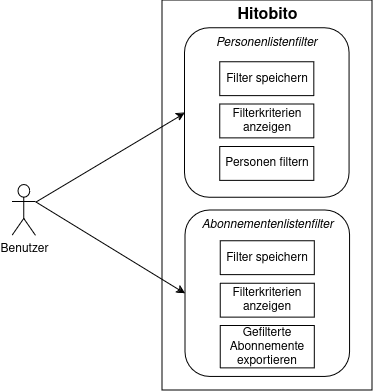
\includegraphics[width=0.85\textwidth,]{hitobito_use_case_diagram.drawio.png}
   \caption{Hitobito Filter Use Case Diagramm}
\end{figure}


\subsection{Anwendungsfälle}
Aus dem Anwendungsdiagram werden die 4 Use-Cases entnommen und hier im Detail beschrieben.

\begin{table}[h!]
   \begin{tabular}{|L{0.3\textwidth}|L{0.6\textwidth}|}
       \hline
       \rowcolor{puzzleblue} \multicolumn{2}{|l|}{\color{white}\textbf{Filter speichern}} \\[4pt]
       \hline
       Kurzbeschreibung & Der Benutzer kann die ausgewählten Fitlerkriterien speichern. \\
       \hline
       Vorbedingungen & 
       \begin{itemize}
         \item Der Benutzer besitzt die nötigen Rechte um eine Filter zu erstellen
         \item Mind. ein Filterkriterium wurde ausgewählt
       \end{itemize} \\
       \hline
       Ablauf & \begin{enumerate}
         \item Benutzer benennt den Filter, optional und nur bei Personenliste
         \item Benutzer klickt auf speichern
       \end{enumerate}  \\
       \hline
       Resultat & Der Filter wurde in der Datenbank persistiert und ein Success-Alert wird ausgegeben. \\
       \hline
   \end{tabular}
   \caption{Anwendungsfall: Filter speichern}
\end{table}

\newpage

\begin{table}[h!]
   \begin{tabular}{|L{0.3\textwidth}|L{0.6\textwidth}|}
      \hline
      \rowcolor{puzzleblue} \multicolumn{2}{|l|}{\color{white}\textbf{Filterkriterien anzeigen}} \\[4pt]
      \hline
      Kurzbeschreibung & Der Benutzer kann die Filterkriterien der gespeicherten Filter einsehen. \\
      \hline
      Vorbedingungen & 
      \begin{itemize}
         \item Der Benutzer hat einen Filter gespeichert
      \end{itemize}  \\
      \hline
      Ablauf & \begin{enumerate}
      \item Navigiert zum Filter
      \end{enumerate}  \\
      \hline
      Resultat & Die Filterkriterien werden dem Benutzer angezeigt. \\
      \hline
   \end{tabular}
   \caption{Anwendungsfall: Filterkriterien anzeigen}
\end{table}

\begin{table}[h!]
   \begin{tabular}{|L{0.3\textwidth}|L{0.6\textwidth}|}
      \hline
      \rowcolor{puzzleblue} \multicolumn{2}{|l|}{\color{white}\textbf{Personen filtern}} \\[4pt]
      \hline
      Kurzbeschreibung & Der Benutzer kann die definierten Personenlistenfilter auf eine Liste von Personen 
      anwenden. \\
      \hline
      Vorbedingungen & \begin{itemize}
         \item Benutzer besitzt Rechte um auf eine Personenliste zuzugreifen
         \item Benutzer hat einen Personenlistenfilter für diese Liste gespeichert
         \end{itemize}  \\
      \hline
      Ablauf & \begin{enumerate}
      \item Benutzer Navigiert zum Personenlistenfilter
      \item Benutzer klickt auf Filternamen
      \end{enumerate}  \\
      \hline
      Resultat & Die Personen in der Personenliste werden gefiltert und dem Benutzer angezeigt. \\
      \hline
   \end{tabular}
   \caption{Anwendungsfall: Personen filtern}
\end{table}

\newpage

\begin{table}[h!]
   \begin{tabular}{|L{0.3\textwidth}|L{0.6\textwidth}|}
      \hline
      \rowcolor{puzzleblue} \multicolumn{2}{|l|}{\color{white}\textbf{Gefilterte Abonnemente exportieren}} \\[4pt]
      \hline
      Kurzbeschreibung & Der Benutzer kann die Abonnemente als PDF, CSV, Excel, etc. exportieren, dabei werden
      die gesetzten Abonnementenfilter auf diesen Export angewendet. \\
      \hline
      Vorbedingungen & \begin{itemize}
         \item Benutzer hat Rechte um Abonnemente zu bearbeiten
         \item Benutzer hat einen Abonnementenfilter gespeichert
         \end{itemize}  \\
      \hline
      Ablauf & \begin{enumerate}
      \item Benutzer zum Abonnementenfilter
      \item Benutzer wählt Zieldatei aus Dropdown aus
      \item Benutzer exportiert Abonnementenliste
      \end{enumerate}  \\
      \hline
      Resultat & Die Personen in der Personenliste werden gefiltert und dem Benutzer angezeigt. \\
      \hline
   \end{tabular}
   \caption{Anwendungsfall: Gefilterte Abonnemente exportieren}
\end{table}

\newpage

\section{Systemkonzept}
Bei dieser Arbeit wird mit einem bestehenden System gearbeitet, dieses muss entsprechend angepasst werden. 
Um die nötigen Anpassungen besser sichtbar zu machen, wird im folgenden Abschnitt gezeigt, welche Services von den 
Anpassungen betroffen, was der aktuelle Stand der Logik und was mögliche Konzepte für die Erweiterung sind. Danach wird aufgrund
eines Variantenentscheids eine Lösungsvariante ausgearbeitet und als Plan für das PoC definiert.

\begin{figure}[h]
   \centering
   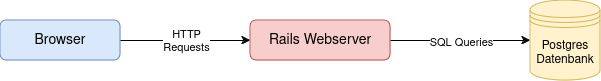
\includegraphics[width=1\textwidth,]{hitobito_systemarchitektur.drawio.png}
   \caption{Services}
\end{figure}

\subsection{Betroffene Services}
Hitobito wird hauptsächlich in zwei Services unterteilt, der Rails Applikation und der Postgres Datenbank.

\textbf{Rails Applikation / Webserver}

Die Rails Applikation verwaltet die Business Logik von Hitobito. Die Änderungen / Erweiterugnen dieser Arbeit
werden alle in diesem Service vorgenommen. Je nach Kunde werden hier Code Teile aus den definierten Wagons verwendet.
In dieser Arbeit wird jedoch ausschliesslich der Core und der Generic Wagon angepasst.

\textbf{Postgres Datenbank}

Die Datenbank von Hitobito läuft auf Postgres. Sämtliche Abfragen auf die Postgres Datenbank werden via SQL-Queries
gemacht. Active Records is das ORM (Object Relational Mapping) welches verwendet wird.

\newpage

\subsection{Status quo}

\textbf{Personlistfilter}

\begin{figure}[h]
   \centering
   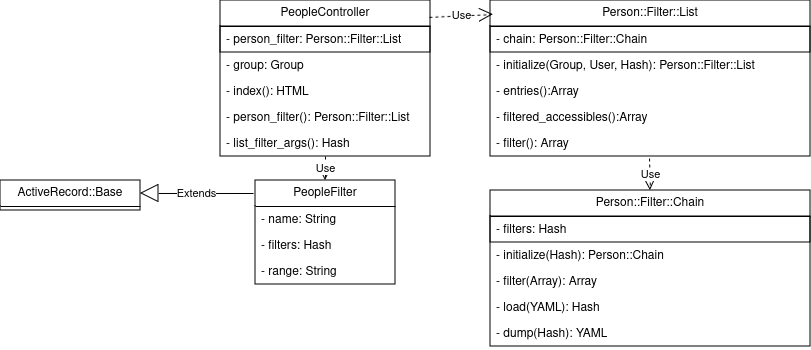
\includegraphics[width=1\textwidth,]{hitobtio_personlist_filter_classstructure.drawio.png}
   \caption{Klassenstruktur Personenlistenfilter}
\end{figure}

In der Abbildung oben ist die Klassenstruktur der Personenlistenfilterlogik zu sehen. Wenn der Benutzer einen Filter-Request
absetzt trifft dieser erstmals auf die \texttt{index} Methode im PeopleController. In dieser ruft der Controller klassenintern die Methode
\texttt{person\_filter} auf. Darin wird eine neue Instanz der \texttt{Person\:\:Filter\:\:List} erstellt und die Filterparameter übergeben.
Die Parameter werden über die Methode \texttt{list\_filter\_args} geholt. Wurde schon ein Fitler abgespeichert, holt sich die Methode
die persistierte Instanz der \texttt{PeopleFilter} Klasse und zieht die Parameter aus dem Attribut \texttt{filters}. Ist noch kein Filter definiert
übergibt die Methode die Parameter des Requests der Instanz. 

Die \texttt{Person\:\:Filter\:\:List} sorgt mit \texttt{filtered\_acessibles} dafür das nur Daten zurückommen, auf welche der Benutzer
Zugriff hat. Die Methode \texttt{filter} ruft intern eine Instanz von \texttt{Person\:\:Filter\:\:Chain} auf und gibt mit durch die Methode \texttt{filter} die
gefilterten Daten zurück.

Um diese Chain später in dem PeopleFilter model zu speichern, überschreibt die Klasse \texttt{Person\:\:Filter\:\:Chain} die \texttt{load} und \texttt{dump} Methode
von Active Rails, um später die Filter Parameter selbständig in einen Hash zu transformieren.

\newpage

\textbf{Abonnementenfilter}
\begin{figure}[h]
   \centering
   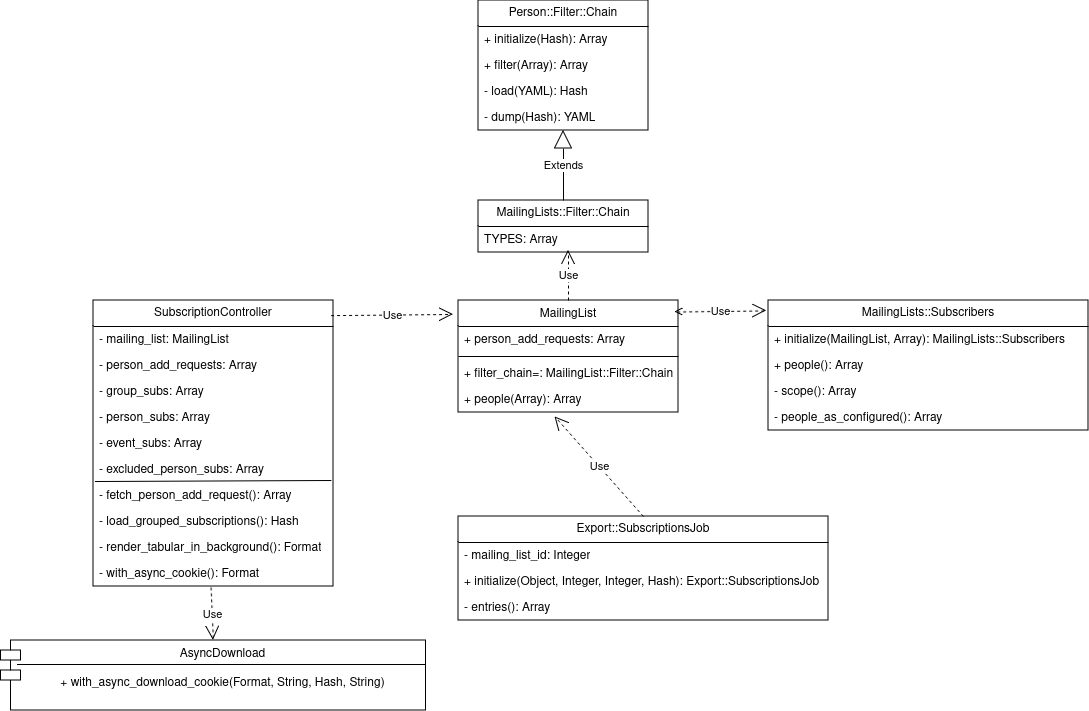
\includegraphics[width=1\textwidth,]{hitobito_subscription_filter.drawio.png}
   \caption{Klassenstruktur Personenlistenfilter}
\end{figure}

In der Klassenstruktur des Abonnementenfilters trifft ein Request des Benutzers zuerst auf die \texttt{index} Action im SubscriptionController. 
Danach wird \texttt{fetch\_person\_add\_request} aufgerufen welche auf die MailingListe zugreift um die \texttt{add\_requests} zu fetchen. Danach wird durch
die Methode \texttt{load\_grouped\_subscriptions} die einzelnen subscribers geladen. Diese werden dann in der Filterungsansicht angezeigt. 

Die Filterung selbst wird nur beim Export von Abonnementen gemacht. Wenn der Benutzer ein CSV der Abonnemente herunterlädt, trifft der Request wieder auf die
\texttt{index} Action im SubscriptionController. Als nächstes wird durch die Methode \texttt{render\_tabular\_in\_background} ein weiterer Aufruf zur 
\texttt{with\_async\_download\_cookie} Methode gemacht, welche sich im Module \texttt{AsyncDownload} befindet. Diese Methdoe lädt das CSV herunter. 
Die Daten dafür bekommt die Methode vom \texttt{Export\:\:SubscriptionsJob} welcher mit der Methode \texttt{entries} die MailingListe aufruft und 
darin durch die Methode \texttt{people} eine Instanz der Klasse \texttt{MailingLists::Subscribers} erstellt. Die Klasse 
holt sich durch \texttt{people\_as\_configured} die gefilterten Abonnemente. Die Filterung geschieht durch einen Call zurück zur Mailingliste welche
dann durch die \texttt{filter\_chain} Methode die Klasse \texttt{MailingLists::Filter::Chain} aufruft. Die Filterung funktioniert von hier an ähnlich wie
bei den Personenlisten, da \texttt{MailingLists::Filter::Chain} von {Person::Filter::Chain} erbt. Mit den gefilterten Abonnementen wird \texttt{scope} aufgerufen
welches schlussendlich doppelte Abonnemente entfernt und zurückgibt. Anhand der gefetchten Daten kann der CSV Export vom \texttt{AsyncDownload} Modul abgeschlossen werden.

\subsection{Lösungsvarianten}
In diesem Abschnitt werden Lösungsvariantent für diese Arbeit definiert. Es sind Grobkonzepte welche genug Informationen darstellen, um eine
Evaluation jeder Variante durchzuführen.

\textbf{Lösungsvariante 1}

\begin{figure}[h]
   \centering
   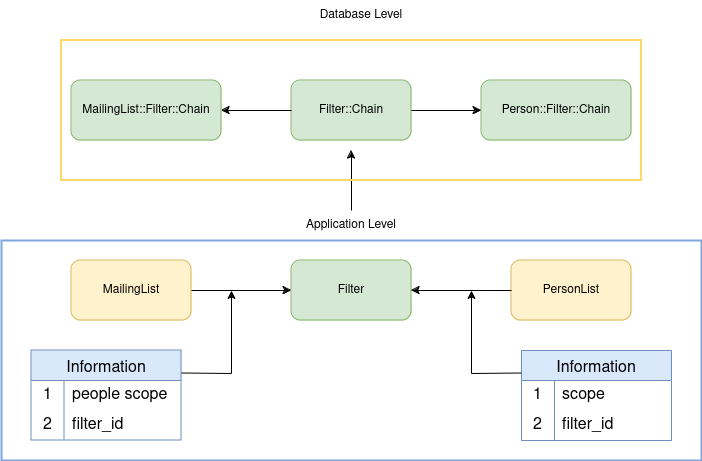
\includegraphics[width=1\textwidth,]{filter_concept_1.drawio.png}
   \caption{Neues Filterkonzept 1}
\end{figure}

Die Idee dieser Variante ist, dass die Filterung selbst nur noch über eine Klasse und ein Modell gelöst wird. Die Klasse Filter soll dabei
die nötigen Parameter entgegennehmen und die neue Entität Filter\:\:Chain aufrufen. Hier handelt es sich um das Parent Modell der MaillingList\:\:Filter\:\:Chain
und der Person\:\:Filter\:\:Chain. Diese Beziehung könnte auf Datenbanklevel mit einer Single Table Inheritance Strategie realisiert werden.
Ziele dieser Lösungsvariante ist den Prozess der Filterung auf eine Klasse zu reduzieren. 

\newpage

\textbf{Lösungsvariante 2}

\begin{figure}[h]
   \centering
   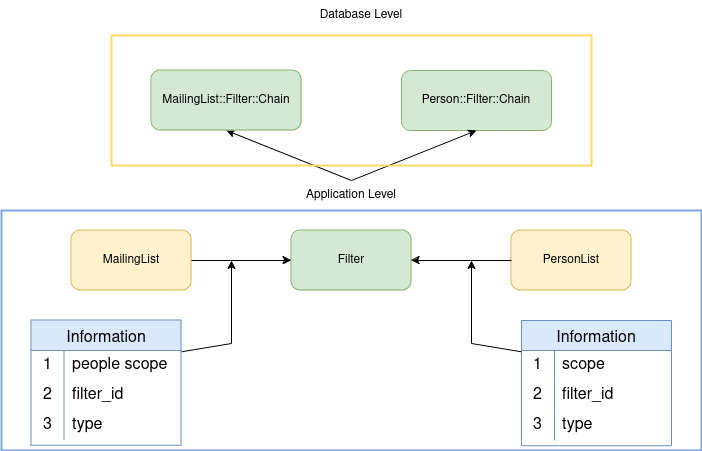
\includegraphics[width=1\textwidth,]{filter_concept_2.drawio.png}
   \caption{Neues Filterkonzept 2}
\end{figure}

Die Lösungvariante 2 ist ähnlich aufgebaut wie die erste. Allerdings wird in dieser Varainte auf die Single Table Inheritance Strategie verzichtet.
Stattdessen soll mit eine Attribute "type" entschieden werden von welchem Typ die Anfrage für eine Filterung kommt. Die Filterklasse entscheidet dann
auf welchen Table sie die SQL-Abfrage richten muss und fetcht die Daten.  

\newpage

\textbf{Lösungsvariante 3}

\begin{figure}[h]
   \centering
   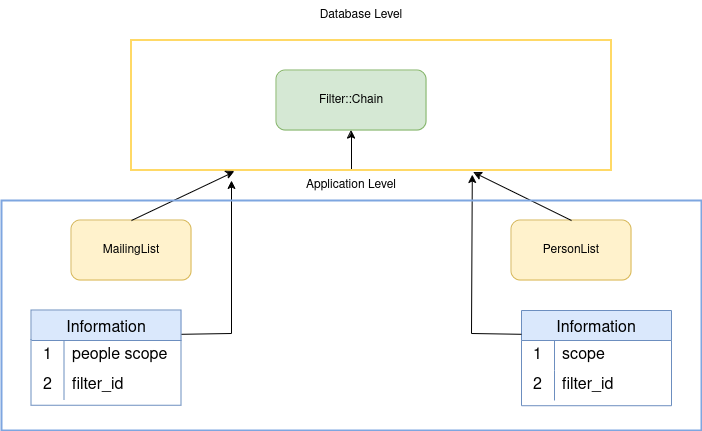
\includegraphics[width=1\textwidth,]{filter_concept_3.drawio.png}
   \caption{Neues Filterkonzept 3}
\end{figure}

Diese Variante lässt den Applicationlayer bestehen wie bisher, es werden keinen neuen Klassen implementiert.
Allerdings greifen die MailingList und die PersonList nun direkt auf ein neues Model zu, der Filter\:\:Chain. Diese 
beinhaltet die einen Zusammenzug der Filterdaten die gespeichert wurden. Dazu muss das \texttt{filter\_chain} Attribut und die People\:\:Filter Entitäten 
in diesen Table migriert werden. Die Information über den Typ nach welchem gefiltert wird, ist nicht mehr nötig da die Filterkriterien direkt mit der Filter ID
vom Table geholt werden können.

\newpage

\subsection{Variantenentscheid}

Um eine geeignete Entscheidung für eine der beschriebenen Lösungsvariantetn zu treffen, wird eine Bewertungsmatrix verwendet welche
jede Lösungsvarainte anhand definierter Kriterien beurteilt. Die Kriterien können mit Punkten von 1 bis 10 bewertet werden, wobei 1 Punkt für das Nicht-Erfüllen
eines Kriteriums und 10 für das Erfüllen des Kriteriums steht. 

Folgende Kriterien wurden definiert:

\begin{table}[h!]
   \begin{tabular}{|L{0.2\textwidth}|L{0.3\textwidth}|L{0.2\textwidth}|L{0.2\textwidth}|}
      \hline
      \rowcolor{puzzleblue}{\color{white} \textbf{Kriterium}} & \color{white}\textbf{Beschreibung} & \color{white}\textbf{1 Punkt} & \color{white}\textbf{10 Punkte} \\[2pt]
      \hline
      Zeitaufwand & Wie viel Zeit wird für die Implementation benötigt? 
      & Grosser Zeitaufwand, IPA ist mit diesem Konzept nicht umsetzbar & Kleiner Zeitaufwand, IPA ist problemlos umsetzbar. \\
      \hline
      Einführung & Ist das Konzept einfach in die produktive Umgebung einzuführen? Müssen Migrationen vorgenommen werden?
       & Einführung in produktive Umgebung ist unmöglich & Einführung in produktive Umgebung ist problemlos möglich.\\
      \hline
      Wissen & Kann der Kandidate mit der Umsetzung des Konzeptes etwas lernen?
      & Kandidat lernt nichts neues dazu & Es kann neues Wissen erarbeitet werden\\
      \hline
      Performance & Ist das Konzept performant? Spart das Konzept Zeit / Requests? 
      & Konzept ist nicht performant, Filterungen werden durch Implementation deutlich langsamer 
      & Hohe Performance, es kann viel Zeit durch die Implementation des Konzepts gespart werden.\\
      \hline
   \end{tabular}
   \caption{Variantenentscheid Kriterien}
\end{table}

\newpage{}

\textbf{Bewertungen}

Im folgenden Abschnitt werden den definierten Kriterien Gewichtungen hinzugefüht, da nicht jedes Kriterium gleich wichtig für
diese IPA ist.

\textbf{Gewichtungen in \%}

\begin{itemize}
   \item \textbf{Zeitaufwand 40\%:} Um eine funktionelle Lösung am Ende der IPA aufweisen zu können, wird dem Zeitaufwand eine hohe Gewichtung zugerodnet
   \item \textbf{Einführung 15\%:} Es ist wichtig eine Lösung zu implementieren welche schnell ihren Weg in die produktive Umgebung findet, da die Einführung von der IPA ausgenommen ist, wird diesem Kriterium eine geringere Gewichtung zugeordnet.
   \item \textbf{Wissen 30\%:} Damit von der IPA profitiert werden kann, sollte von der Kandidat stets eine Wissenserweiterung durch deren Umsetzung erlangen. 
   \item \textbf{Performance 15\%: } Ist eine Applikation zu langsam und benötigt mehrere Minute bis sie Resultate geladen hat, kann das den Benutzer schnell vor den Kopf stossen und dafür führen das dieser die Applikation in Zukunft nicht mehr verwendet.
\end{itemize}

\textbf{Lösungsvariante 1}

\begin{table}[h!]
   \begin{tabular}{|L{0.2\textwidth}|L{0.2\textwidth}|L{0.6\textwidth}|}
      \hline
      \rowcolor{puzzleblue}{\color{white} \textbf{Kriterium}} & \color{white}\textbf{Bewertung} & \color{white}\textbf{Beschreibung}\\[2pt]
      \hline
      Zeitaufwand & 2 & Grösster Zeitaufwand, Konzeption mit den meisten Neuimplementationen. \\
      \hline
      Einführung & 4 & Einführung möglich, es sollten keine grossen Schwierigkeiten auftreten \\
      \hline 
      Wissen & 10 & Durch viele Neuimplementationen kann hier am meisten profitiert werden. \\
      \hline
      Performance & 5 & Performance kann mit Sicherheit beibehalten werden. \\
      \hline
   \end{tabular}
   \caption{Bewertung Lösungsvariante 1}
\end{table}

\newpage

\textbf{Lösungsvariante 2}

\begin{table}[h!]
   \begin{tabular}{|L{0.2\textwidth}|L{0.2\textwidth}|L{0.6\textwidth}|}
      \hline
      \rowcolor{puzzleblue}{\color{white} \textbf{Kriterium}} & \color{white}\textbf{Bewertung} & \color{white}\textbf{Beschreibung}\\[2pt]
      \hline
      Zeitaufwand & 4 & Mittlerer Zeitaufwand, eine Neuimplementation \\
      \hline
      Einführung & 5 & Einführung problemlos möglich, es werden keine Migrationen benötigt \\
      \hline 
      Wissen & 8 & Durch die Neuimplementation einer Filterklasse kann profitiert werden, Punktabzug aufgrund der nicht vorhandenen Umsetzung der Single Table Inheritance \\
      \hline
      Performance & 5 & Performance kann mit Sicherheit beibehalten werden. \\
      \hline
   \end{tabular}
   \caption{Bewertung Lösungsvariante 2}
\end{table}

\textbf{Lösungsvariante 3}

\begin{table}[h!]
   \begin{tabular}{|L{0.2\textwidth}|L{0.2\textwidth}|L{0.6\textwidth}|}
      \hline
      \rowcolor{puzzleblue}{\color{white} \textbf{Kriterium}} & \color{white}\textbf{Bewertung} & \color{white}\textbf{Beschreibung}\\[2pt]
      \hline
      Zeitaufwand & 4 & Mittlerer Zeitaufwand, keine Neuimplementationen jedoch müssen Migrationen gemacht werden. \\
      \hline
      Einführung & 8 & Durch die Migration beider Tables ist das Potential für Schwierigkeiten bei der Einführung hier am Grössten. \\
      \hline 
      Wissen & 3 & Neues Wissen wird kaum erlangt, als Bonus gilt lediglich das Schreiben einer Migration. \\
      \hline
      Performance & 7 & Performance könnte durch erhöhte Aufrufe auf einen Table gefährdet sein. \\
      \hline
   \end{tabular}
   \caption{Bewertung Lösungsvariante 3}
\end{table}

\newpage

\begin{landscape}
   \begin{table}[h!]
      \begin{tabular}{|m{0.17\textwidth}|L{0.17\textwidth}|L{0.17\textwidth}|L{0.17\textwidth}|L{0.17\textwidth}|L{0.17\textwidth}|L{0.17\textwidth}|L{0.17\textwidth}|}
         \hline
         \rowcolor{puzzleblue} \multicolumn{2}{|l|}{} & \multicolumn{2}{|l|}{\color{white} \textbf{Variante 1}} & \multicolumn{2}{|l|}{\color{white} \textbf{Variante 2}} & \multicolumn{2}{|l|}{\color{white}\textbf{Variante 3}} \\[2pt]
         \hline
         \multirow{2}{*}{Kriterium} & \multirow{2}{*}{Gewichtung} & \multirow{2}{*}{Ungewichtet} & \multirow{2}{*}{Gewichtet} & \multirow{2}{*}{Gewichtet} & \multirow{2}{*}{Gewichtet} & \multirow{2}{*}{Ungewichtet} & \multirow{2}{*}{Gewichtet} \\ [10pt]
         \hline
         \multirow{2}{*}{Zeitaufwand} & \multirow{2}{*}{40\%} & \multirow{2}{*}{2} & \multirow{2}{*}{0.8} & \multirow{2}{*}{4} & \multirow{2}{*}{1.6} & \multirow{2}{*}{4} & \multirow{2}{*}{1.6} \\[10pt]
         \hline
         \multirow{2}{*}{Einführung} & \multirow{2}{*}{15\%} & \multirow{2}{*}{4} & \multirow{2}{*}{0.6} & \multirow{2}{*}{5} & \multirow{2}{*}{0.75} & \multirow{2}{*}{8} & \multirow{2}{*}{1.2} \\[10pt]
         \hline 
         \multirow{2}{*}{Wissen} &  \multirow{2}{*}{30\%} & \multirow{2}{*}{10} & \multirow{2}{*}{3} & \multirow{2}{*}{8} & \multirow{2}{*}{2.4} & \multirow{2}{*}{3} & \multirow{2}{*}{0.9} \\[10pt]
         \hline
         \multirow{2}{*}{Performance} & \multirow{2}{*}{15\%} & \multirow{2}{*}{5} & \multirow{2}{*}{0.75} & \multirow{2}{*}{5} & \multirow{2}{*}{0.75} & \multirow{2}{*}{7} & \multirow{2}{*}{1.05} \\[10pt]
         \hline
         \multirow{2}{*}{Total} & \multirow{2}{*}{100\%} &  \multirow{2}{*}{21} & \multirow{2}{*}{5.15} & \multirow{2}{*}{19} & \multirow{2}{*}{5.5} & \multirow{2}{*}{22} & \multirow{2}{*}{4.75} \\[10pt]
         \hline
      \end{tabular}
      \caption{Nutzwertanalyse}
   \end{table}

\textbf{Fazit}

Aus der Nutzwertanalyse kann geschlossen werden, dass sich die Variante 2 am Besten für die IPA eignet. Sie ist in der nötigen Zeit umsetzbar,
bietet die Möglichkeit zum Wissensausbau, kann schnell eingeführt werden und wird vorausichtlich an der Performance nichts verändern.

\end{landscape}

\newpage

\begin{landscape}
   \subsection{Ausarbeitung}
   Im Diagramm unten ist die augearbeitete Klassenstruktur zu sehen. Alles was grün markiert ist, wurde neu
   hinzugefügt oder erweitert, alles was rot ist wurde entfernt. Es wird ein neues Modul geben, das \texttt{ModelFilter} Modul
   welches die Filterprozesse übernimmte welche vorher von der \texttt{Person::Filter::List} und \texttt{MailingLists::Subscribers} Klasse
   durchgeführt wurden. 

   \begin{figure}[h]
      \centering
      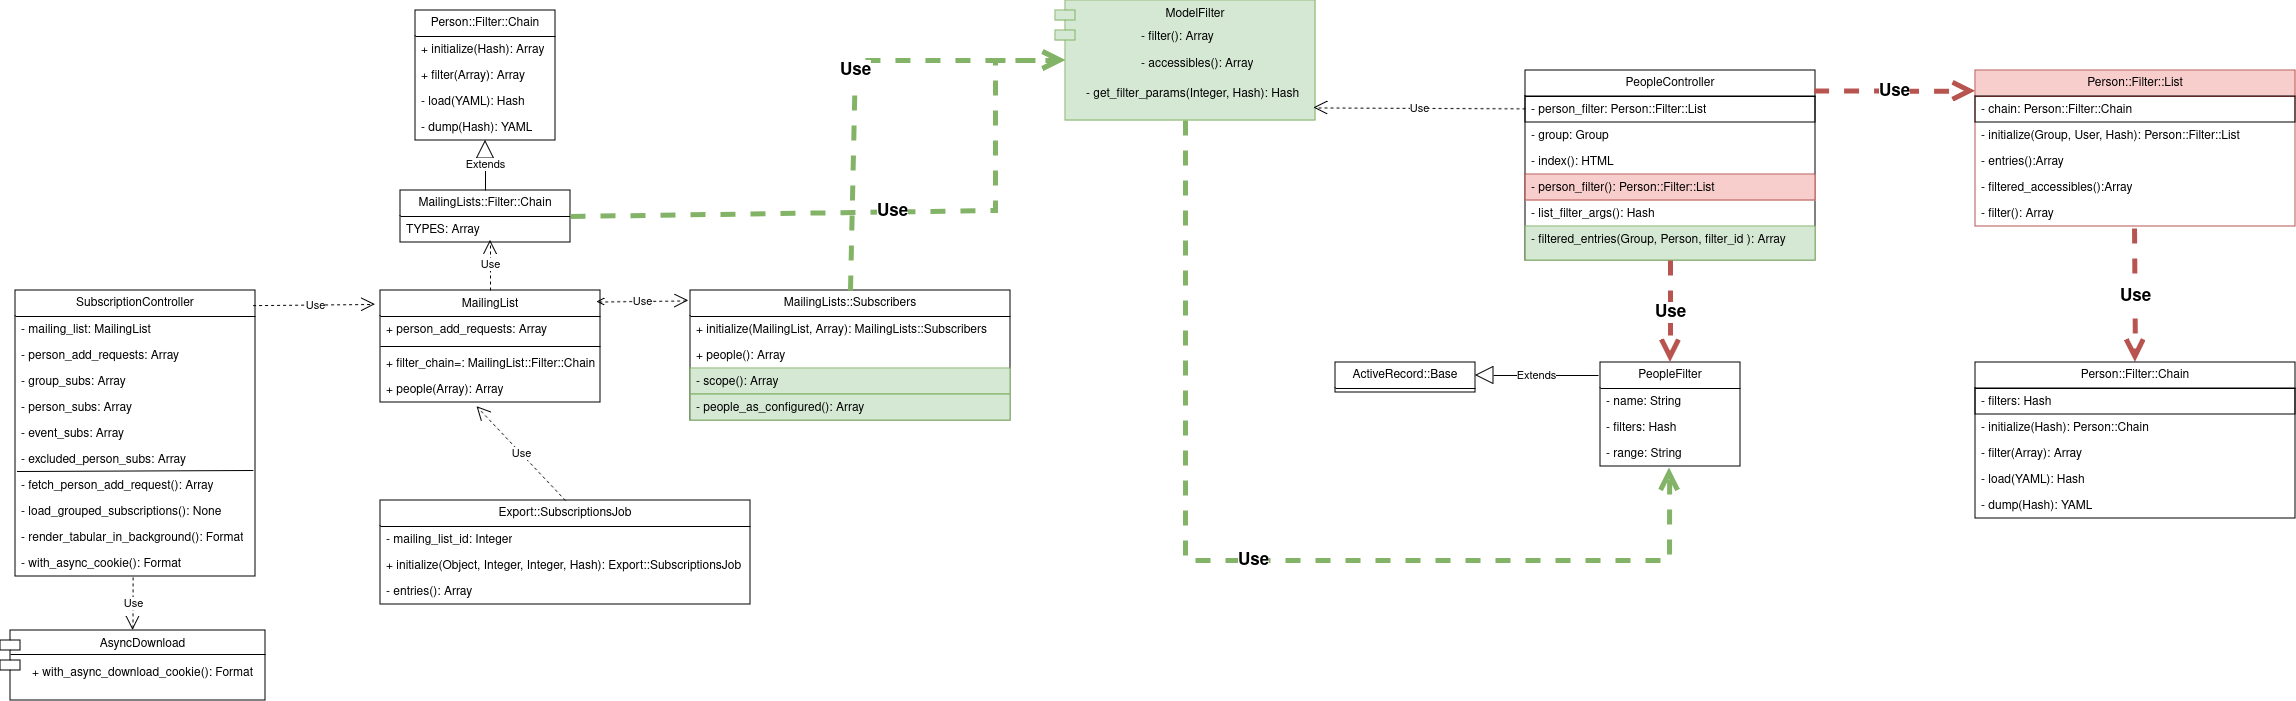
\includegraphics[width=1.5\textwidth,]{hitobito_reworked_class_structure.drawio.png}
      \caption{Ausgearbeitete Klassenstruktur}
   \end{figure}

   Um diese Klassen und Funktionen zu ersetzen, sind drei Methoden im neuen Modul angedacht. Zum einen die \texttt{filter} Methode welche 
   auf die \texttt{Person\:\:Filter\:\:Chain} oder \texttt{MailingList\:\:Filter\:\:Chain} zugreifen wird, um den gegebenen Scope zu filtern.
   Damit nicht unberechtig auf Datensätze zugegriffen wird, gibt es zusätzlich die Methode \texttt{accessibles} welche die Daten vor der Fitlerung auf
   die Berechtigungen des Benutzers prüft. Zuletzt gibt es die Methode \texttt{get\_filter\_parameters} diese Methode ist dazu angedacht, um auf das \texttt{PeopleFilter}
   Model zuzugreifen und die Filterkriterien aus diesem herauszuholen, wenn ein solcher Filter existiert.


\end{landscape}

\subsection{Gems}
TODO: Describe

\section{Sicherheitskonzept}
Um die Sicherheit im Umbau der Filter sicherzustellen wird ein Sicherheitskonzept
benötigt. Das Ziel dieses Konzeptes ist es mögliche Angriffe aufzuführen
und die Blockade dieser Angriffe zu dokumentieren. 

\subsection{SQL-Injection}
Die Einzigen Userinputs welche in dieser IPA auftreten sind die Textinputs welche im Filter
ausgewählt werden können. Da die Eingabe des Users nicht direkt in die Postgres Datenbank gespeichert wird,
ist diese Eingabe nicht für eine SQL-Injection gefährdet. Selbst wenn die SQL-Abfrage direkt gemacht würde,
verhindert das ORM ActiveRecord mit seinen Standardmethoden, dass schädliche Eingaben abgespeichert werden.
Dies geschieht unter anderem durch escapen der Strings.

\subsection{Cross-Site Scripting}
Da in diesem Feature Userinputs an das Rails-Backend gesendet werden muss die Cross-Site Scripting Attacke ebenfalls
berücksichtig werden. Rails selbst bietet dafür einen eingebauten Abwehrmechanismus. Wenn der User eine XSS-Attacke ausführen möcht,
indem er in einem der Filterinputs folgende Javascript Eingaben macht:

\begin{verbatim}
   <h2>Welcome <script>alert("This is a XSS attack!")</script></h2>
\end{verbatim}

Standardmässig escaped Rails diese Eingaben und ändert die special characters. So wird aus der Eingabe oben:

\begin{verbatim}
   <h2>Welcome &lt;script&gt;alert\
   (&quot;This is a XSS attack!&quot;)&lt;/script&gt;</h2>
\end{verbatim}

\newpage

\subsection{URL Interpretation}
Bei der URL-Interpretation fabriziert der Angreifer eine URL um damit auf die persönlichen
Daten eines Benutzers zuzugreifen. Dabei kann der Angreifer versuchen die URL zu erraten. 
Dieser Angriff wird in Hitobito mit dem Gem \texttt{can-can-can} verhindert. Mit diesem Gem wird sichergestellt,
das der Absender der Anfrage die nötigen Berechtigungen für das Einsehen der Informationen hat. Die Prüfung der Berechtigungen sieht wie folgt
aus: 

\begin{verbatim}
   class Ability include CanCan::Ability

   def define_root_abilities
    can :manage, :all
    # root cannot change her email, because this is what makes her root.
    cannot :update_email, Person do |p|
      p.root?
    end
  end
\end{verbatim}

\subsection{Kommunikation HTTP/S}
Die Umgebungen auf der Integration und Produktion kommunizieren via HTTPS. Somit ist
die verschlüsselte Kommunikation beim Transfer von produktiven Daten gesichert.

\section{Fehlerbehandlungskonzept}
Bei der Entwicklung und während der Laufzeit können stets Fehler oder nicht vorgesehene Probleme entstehen.
Im folgenden Abschnitt wird dokumentiert, wie mit diesen Fällen umgegangen wird.

\subsection{Nutzereingabe}
Bei der Nutzereingabe des Users werden keine möglichen Exceptions erwartet. Der Benutzer kann im Filter, in der Suche nach einem
bestimmten Text alles eingeben, ohne Einschränkungen. Mögliche Angriffe über Injections werden nach dem definierten
Sicherheitskonzept abgehandelt.

\subsection{Laufzeitfehler}
Tritt in der Applikation ein Laufzeit Fehler auf wird dies sowohl in den Logs wie in der Sentry
Umgebung von Hitobito aufgezeigt. Im Sentry werden zusätzlich die aufgetretenen Execptions gesammelt, um 
den Entwicklern eine Übersicht über allfällige Bugs zu geben. Gesammelte Exceptions können einem Entwickler
zugewiesen oder wenn sie gefixed wurden, vom Sentry entfernt werden. Für diese IPA ist keine Modifizierung an der 
Sentry Umgebung nötig.

\subsection{Exception Handling}
Ruby benötigt kein Exception Handling wie es in anderen Sprachen der Fall ist. Exceptions werden durch Conditionals
abgehandelt, reicht das nicht werden die Exceptions wie die Laufzeitfehler behandelt und erscheinen im Sentry.

\section{Testkonzept}
\subsection{Testinfrastruktur}
In dieser IPA unterscheiden wir drei Arten von Tests:

\begin{itemize}
   \item \textbf{Controller Tests:} Tests die Action eines Controllers
   \item \textbf{Domain Tests:} Testet die Funktion eines Domain-Models
   \item \textbf{Manuelles Testen:} Testet das gesamte Feature
\end{itemize}

Hitobito verwendet für das Ausführen lokaler Tests RSpec 3.13.0. Für die manuellen Tests wird Firefox 80.0 (64-bit) verwendet. Als Gerät wird ein Laptop mit Pop!\_OS 22.04 LTS verwendet.
Um während der Entwicklung die Funktionalität der Applikation sicherzustellen werden die bereits bestehenden Tests im Hitobito ausgeführt und somit die Controller sowie Domain Tests abgedeckt.
Es werden in dieser Arbeit somit keine neuen Domain oder Controller Tests geschrieben.

\newpage

\subsection{Fehlerklassen}

\begin{table}[h!]
   \begin{tabular}{|L{0.2\textwidth}|L{0.4\textwidth}|L{0.4\textwidth}|}
       \hline
       \rowcolor{puzzleblue} \color{white}\textbf{Bezeichnung} & \color{white}\textbf{Fehlerklasse} & \color{white}\textbf{Beschreibung} \\[12pt]
       \hline
       FK0 & Fehlerfrei & Keine Fehler \\
       \hline
       FK1 & Nicht erfolgsgefährdend & Kleine Fehler, beeinträchtigen Funktion nur bedingt. \\
       \hline
       FK2 & Erfolgsgefährdend & Fehler welche die Funktion beeinträchtigen. \\
       \hline
     \end{tabular}
     \caption{Fehlerklassen}
\end{table}

\subsection{Manuelle Tests}
Die manuellen Tests werden lokal, mit den Testdaten von Hitobito durchgeführt. Die Testdaten können in der Hitobito-Konsole
mit \texttt{hit rails wagon seed} eingespielt werden. Mit dem generic Wagon bieten sich drei mögliche User für das Login an:

\begin{table}[h!]
   \begin{tabular}{|L{0.4\textwidth}|L{0.2\textwidth}|L{0.4\textwidth}|}
       \hline
       \rowcolor{puzzleblue} \color{white}\textbf{Username} & \color{white}\textbf{Passwort} & \color{white}\textbf{Berechtigungen}\\[12pt]
       \hline
        admin@hitobito.ch & demo & Administrator mit vollem Zugriff \\
       \hline
       leitung@hitobito.ch & demo &  Rolle Leitung einer lokalen Gruppe\\
       \hline
       mitglied@hitobito.ch & demo & Einfaches Gruppenmitglied \\
       \hline
     \end{tabular}
     \caption{Accounts für manuelle Tests}
\end{table}


Bei den manuellen Tests muss man sich immer mit einer der oben beschriebenen Accounts einloggen.
In den Testszenarien wird der Account mit "Als {Account} anmelden" beschrieben, {Account} steht hierbei als
Platzhalter für den Account des jeweiligen Benutzer. Der Loginablauf ist:

\begin{itemize}
   \item Navigation auf \texttt{localhost:3000/users/sign\_in}
   \item Account Credentials eingeben
   \item Auf Button Anmelden klicken
\end{itemize}

\newpage

\begin{table}[h!]
   \rowcolors{2}{puzzleblue!30}{white}
   \begin{tabular}{|L{0.4\textwidth}|L{0.6\textwidth}|}
       \hline
       \rowcolor{puzzleblue} \multicolumn{2}{|l|}{\color{white}\textbf{Testfall Nr. 1}} \\[12pt]
       \hline
        Testname & Personenliste, gesamte Ebene \\
       \hline
       Testmethode & Manuell \\
       \hline
        Anforderung & Funktionale Anforderung 2 \\
       \hline
       Voraussetzungen & Keine \\
       \hline
       Testszenario & 
       \begin{itemize}
         \item Als Admin anmelden
         \item Mittels Link "Personen" auf Personenliste navigieren
         \item Im Filter "Gesamte Ebene" auswählen
       \end{itemize} \\
       \hline
       Erwartetes Resultat & 
       \begin{itemize}
         \item Alle Personen werden angezeigt
      \end{itemize} \\
      \hline
     \end{tabular}
     \caption{Testfall 1}
\end{table}

\newpage

\begin{table}[h!]
   \rowcolors{2}{puzzleblue!30}{white}
   \begin{tabular}{|L{0.4\textwidth}|L{0.6\textwidth}|}
       \hline
       \rowcolor{puzzleblue} \multicolumn{2}{|l|}{\color{white}\textbf{Testfall Nr. 2}} \\[12pt]
       \hline
        Testname & Personenliste, Carlo Filter \\
       \hline
       Testmethode & Manuell \\
       \hline
        Anforderung & Funktionale Anforderung 2 \\
       \hline
       Voraussetzungen & Ein Filter mit dem Namen "Carlo" wurde erstellt, welche alle User mit dem 
       Vornamen "Carlo" zurückgibt. \\
       \hline
       Testszenario & 
       \begin{itemize}
         \item Als Admin anmelden
         \item Mittels Link "Personen" auf Personenliste navigieren
         \item Im Filter "Carlo" auswählen
       \end{itemize} \\
       \hline
       Erwartetes Resultat & 
       \begin{itemize}
         \item Alle Personen mit Vornamen "Carlo" werden angezeigt
         \item Filternamen wird korrekt dargestellt
      \end{itemize} \\
      \hline
     \end{tabular}
     \caption{Testfall 2}
\end{table}

\newpage

\begin{table}[h!]
   \rowcolors{2}{puzzleblue!30}{white}
   \begin{tabular}{|L{0.4\textwidth}|L{0.6\textwidth}|}
       \hline
       \rowcolor{puzzleblue} \multicolumn{2}{|l|}{\color{white}\textbf{Testfall Nr. 3}} \\[12pt]
       \hline
        Testname & Abonnemente, PDF-Export \\
       \hline
       Testmethode & Manuell \\
       \hline
        Anforderung & Funktionale Anforderung 2 \\
       \hline
       Voraussetzungen & Unter den globalen Bedingungen wurden alle User aufgenommen, welche den Vornamen
       "Carlo besitzen" \\
       \hline
       Testszenario & 
       \begin{itemize}
         \item Als Admin anmelden
         \item Mittels Link "Abonnemente" auf Abonnementenliste navigieren
         \item In der Abonnementenliste das Abo "Bloodaxe Fist" auswählen
         \item Unter Dropdown "Export" PDF auswählen
       \end{itemize} \\
       \hline
       Erwartetes Resultat & 
       \begin{itemize}
         \item PDF wird heruntergeladen
         \item Auf dem PDF befinden sich nur Benutzer mit dem Vornamen "Carlo"
      \end{itemize}\\
      \hline
     \end{tabular}
     \caption{Testfall 3}
\end{table}

\newpage

\begin{table}[h!]
   \rowcolors{2}{puzzleblue!30}{white}
   \begin{tabular}{|L{0.4\textwidth}|L{0.6\textwidth}|}
       \hline
       \rowcolor{puzzleblue} \multicolumn{2}{|l|}{\color{white}\textbf{Testfall Nr. 4}} \\[12pt]
       \hline
        Testname & Abonnemente, Excel-Export \\
       \hline
       Testmethode & Manuell \\
       \hline
        Anforderung & Funktionale Anforderung 2 \\
       \hline
       Voraussetzungen & Unter den globalen Bedingungen wurden alle User aufgenommen, welche den Vornamen
       "Carlo besitzen" \\
       \hline
       Testszenario & 
       \begin{itemize}
         \item Als Admin anmelden
         \item Mittels Link "Abonnemente" auf Abonnementenliste navigieren
         \item In der Abonnementenliste das Abo "Bloodaxe Fist" auswählen
         \item Unter Dropdown "Export" Excel und danach "Adressliste" auswählen
       \end{itemize} \\
       \hline
       Erwartetes Resultat & 
       \begin{itemize}
         \item Excel wird heruntergeladen
         \item Auf dem Excel befinden sich nur Adressen von Benutzern mit dem Vornamen "Carlo"
      \end{itemize}\\
      \hline
     \end{tabular}
     \caption{Testfall 4}
\end{table}

\chapter{Ausführung}
\section{Klassenstruktur}
Während der Umsetzung habe ich mich an der Klassenstruktur im Entwurf orientiert. Obwohl die Grundlage der Implementation diesem Konzept
gefolgt ist, gabe es dennoch gewisse Abweichungen. Entsprechend wurde ein neues Klassendiagramm erstellt:

\begin{landscape}
   \begin{figure}[h]
      \centering
      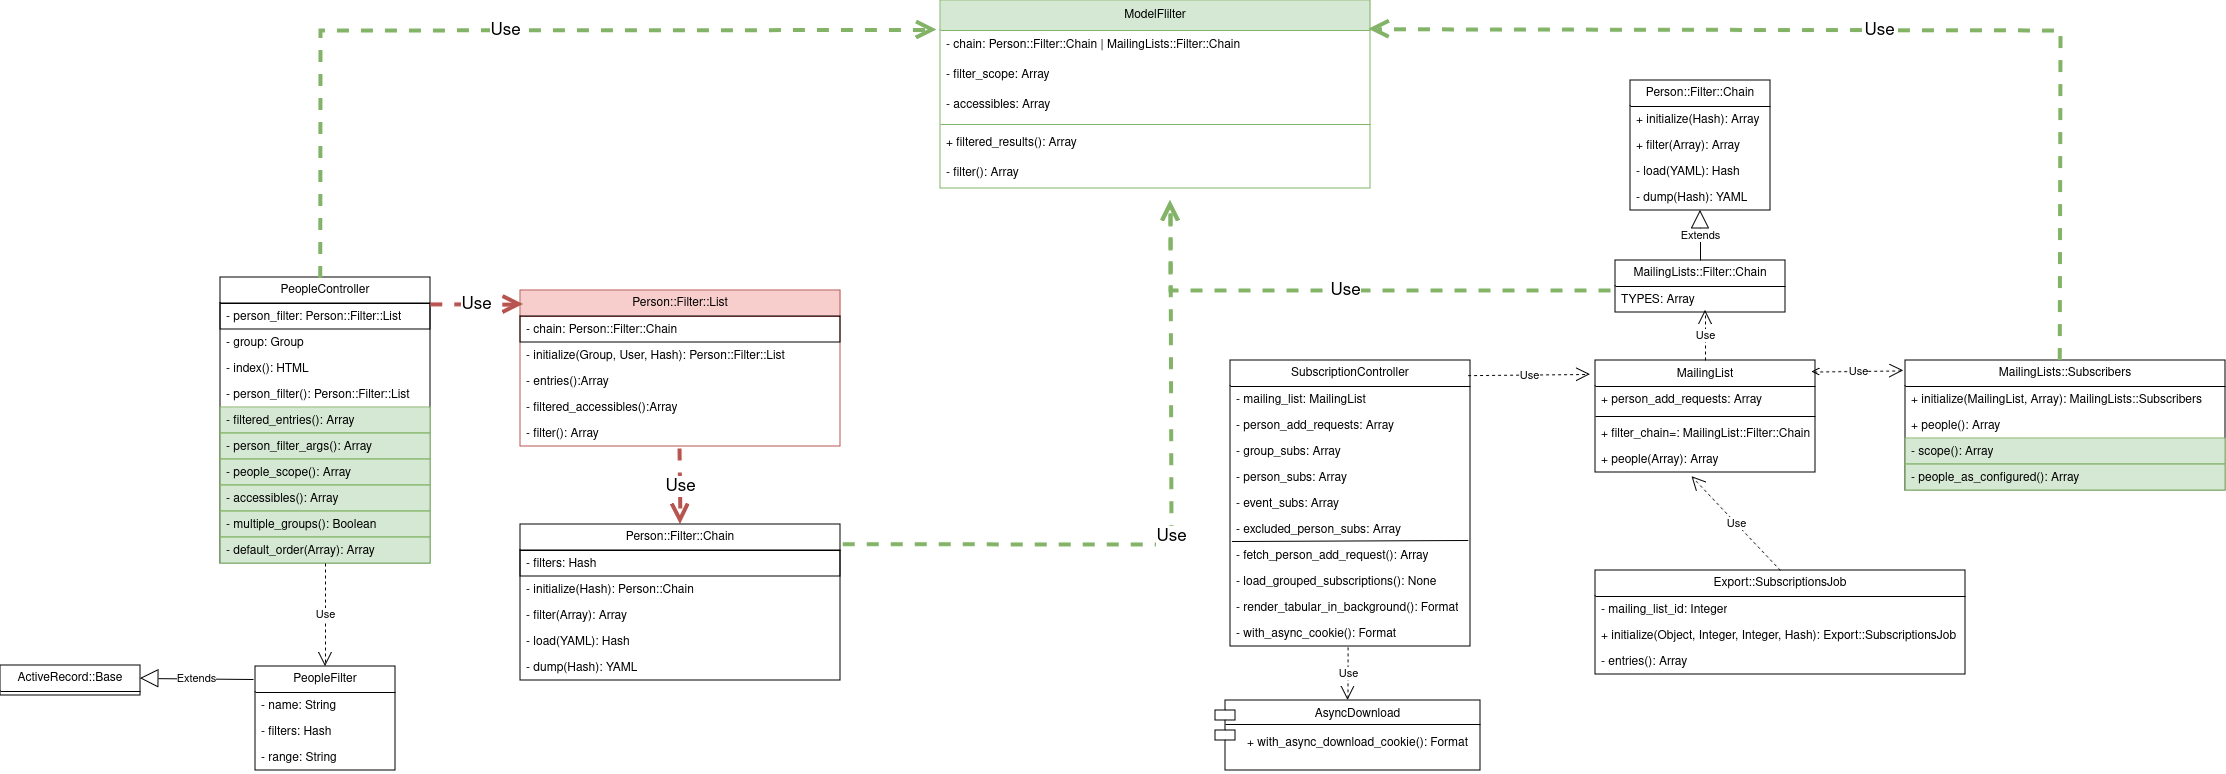
\includegraphics[width=1.5\textwidth,]{hitobito_implemented_class_structure.drawio.png}
      \caption{Klassendiagramm nach Umsetzung}
   \end{figure}

   \subsection{PeopleController}
   Der PeopleController musste mehr erweitert werden als gedacht. Dies lag an der Entscheidung
   jegliche \texttt{People}\-Logik aus dem Filter zu entfernen und in den Controller zu verlagern. Die wichtigste Methode ist \texttt{filtered\_entries}.
   Von dieser Methode aus wird der Aufruf zum \texttt{ModelFilter} gemacht, welcher dann die Filterung übernimmt. Aus dem Filter selbst wurde die Methode
   \texttt{default\_order} übernommen, welche dafür sorgt, dass die Ergebnisse in der richtig sortiert werden. Vorher befand sich die Methode im Filter, sie wurde entfernt da die Sortierung nichts mit der Filterung zu
   tun hat und sich mit der neuen Struktur eine klare Abgrenzung zwischen Filterungssystem und Formatierung der Daten vor dem Zurückstellen ergibt.  
\end{landscape}

\subsection{ModelFilter}
Der \texttt{ModelFilter} kam in der Grössenordnung in der er im Entwurf geplant wurde daher. Anders als geplant wurde er als Klasse nicht als Modul implementiert. Der Grund dafür ist,
das in einer View eine Instanz des Filter benötigt ist, um auf nur ihm bekannte Attribute zuzugreifen. Als Zusatz kam das \texttt{chain}-Argument. Während des Entwickelns kam die Idee auf, dass anstatt einer get-Methode für die Filterchain,
diese direkt vom Controller und der Subscriber-Klasse übergeben werden könnte. So wird das geplante \texttt{type}-Attribut beim Filteraufruf gespart und der Filter wird noch generischer. Dies führt dazu das 
die nicht funktionale Anforderung 1 (Erweiterbarkeit) besser abgedeckt werden kann, denn nun könnten theoretisch jegliche weitere Models mit ihrer eigenen Filterchain an den \texttt{ModelFilter} gegeben werden, welcher nur noch die Filterung selbst durchführt.

\subsection{MaillingLists::Subscribers}
Diese Klasse kam dem Entwurf am nächsten. Es konnte wie geplant die Methoden \texttt{scope} und \texttt{people\_as\_configured} so erweitert werden, dass nur noch der Aufruf zum \texttt{ModelFilter} stattfindet. Die restliche Logik bleibt unverändert. 

\subsection{Person::Filter::List}
Im UML wurde diese Klasse mit rot markiert, da sie nun nicht mehr im Filterprozess der Personenlisten und Abonnementen integriert ist. Um die Funktionalität der Komponenten, welche in dieser IPA nicht berücksichtig trotzdem zu 
gewährleisten und somit die Möglichkeit für manuelles Testing sicherzustellen, wurde die Klasse nicht aus dem Repository entfernt. 

\section{Gems}
In der Analyse der Arbeit wurde aufgeführt welche Gems voraussichtlich in der Arbeit verwendet werden. Dieser Abschnitt klärt, wie die Arbeit mit den genannten Gems funktionierte.

\subsection{can-can-can}
In der Analyse wurde erwartet das mit dem can-can-can Gem gearbeitet werden muss, um nur die Daten in die Filterung aufzunehmen, auf welche der Benutzer Zugriff hat.
Wie während der Implementierung festgestellt wurde, konnte direkt auf ein Array mit den bereits verifizierten Daten zugegriffen werden. Sodurch war eine direkte Interaktion mit dem Gem
nicht mehr nötig.

\subsection{dry-crud}
Das dry-crud Gem wurde ebenfalls nicht direkt verwendet. Die Anpassungen am Controller konnten vollzogen werden, ohne Methoden zu verändern welche durch von diesem Gem betroffen sind.

\section{Unvorhergesehene Änderungen}
In der Umsetzung dieser Arbeit traten Änderungen an Teilen der Applikation auf, welche im Entwurf nicht berücksichtig wurden.

\subsection{application.rb}
Standardmässig inkludiert Rails nur bestimmte Ordner und Dateien in seinem \texttt{load\_path}. Während der Implementation wurde ein neuer Ordner \texttt{filter}
angelegt um die neue Klasse darin zu verwalten. Da diese Klasse nicht im \texttt{load\_path} war musste sie im \texttt{application.rb} hinzugefügt werden:

\begin{verbatim}
   # Custom directories with classes and modules you want to be autoloadable.
   config.autoload_paths += %W( #{config.root}/app/abilities
                                #{config.root}/app/domain
                                #{config.root}/app/domain/filter
                                #{config.root}/app/jobs
                                #{config.root}/app/serializers
                                #{config.root}/app/utils
                            )
\end{verbatim}

\subsection{\_list.html.haml}
Die View welche die Personenliste darstellt, beinhaltete eine Referenz adressiert an die Instanz der \texttt{Person::Filter::List}. Damit die View dennoch für das manuelle Testing verwendete werden kann 
wurde ein Teil der Zeit für die Sicherstellung der Anzeige verwendet. Der Teil der am meisten Aufwand verursachte war die Anpassung des \texttt{FilterNavigation::People} in der View.

\begin{verbatim}
   - content_for(:filter, FilterNavigation::People
   .new(self, @group, @model_filter, @name).to_s)
\end{verbatim}

Dieser Komponent verwaltet die Auswahl des Filers über das UI. Durch das Entfernen der \texttt{Person::Filter::List} aus dem Filterprozess, musste die Refernz der View auf den neuen \texttt{ModelFilter}
geändert werden. Zusätzlich holte dieser Komponent den definierten Name des Personenfilters:

\newpage

\begin{figure}
   \centering
   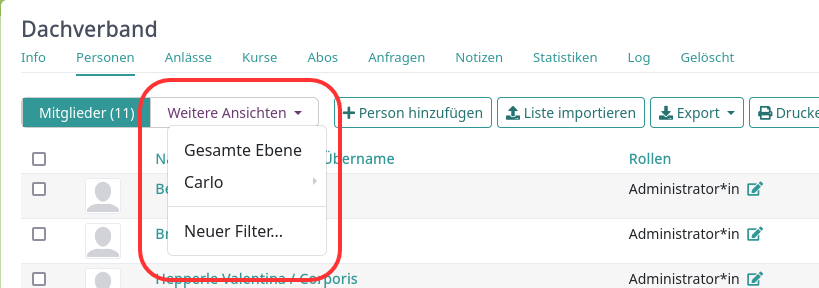
\includegraphics[width=1\textwidth,]{hitobito_named_filtert.drawio.png}
   \caption{Klassendiagramm nach Umsetzung}
\end{figure}

Über diese Referenz. Das das Ziel eine Abgrenzung genau diser Verbindung der Funktionen war, wurde eine Instanzvariable im \texttt{PeopleController} angelegt welche den Namen des Personenlistenfilters speichert
falls dieser existiert:

\begin{verbatim}
   def person_filter_args
    if params[:filter_id]
      filter = PeopleFilter.for_group(group).find(params[:filter_id])
      @name = filter.name
      filter.to_params[:filters]
    else
      params
    end
  end
\end{verbatim}

\section{Testprotokoll}

% Beispiel für Test Tabelle, muess je nachdem angepasst werden

\begin{table}[H]
    \rowcolors{2}{puzzleblue!25}{white}
    \begin{tabular}{|L{0.3\textwidth}|L{0.65\textwidth}|}
        \hline
        \rowcolor{puzzleblue} \multicolumn{2}{|l|}{\color{white}Resultat Testfall Nr. 1}  \\[10pt]
        \hline
        \textbf{Testname} &  \\
        \hline
        \textbf{Testkontext} &  \\
        \hline
        \textbf{Testperson} &  \\
        \hline
        \textbf{Ausführungs Datum} &  \\
        \hline
        \textbf{Testergebnis} &  \\
        \hline
        \textbf{Beschreibung} &  \\ 
        \hline
        \textbf{Fehlerklasse} & \\ 
        \hline
    \end{tabular}
    \caption{Resultat Testfall 1}
\end{table}


\chapter{Einführung}

\chapter{Sprintabschlüsse}

\section{Abschluss Sprint Initialisierung}

\section{Abschluss Sprint Umsetzung}

\section{Abschluss Sprint Finalisierung}


